\documentclass[paper=a4,fontsize=11pt]{scrartcl} % KOMA-article class

\usepackage{comment}
\usepackage[english]{babel}
\usepackage[utf8]{inputenc}
\usepackage[protrusion=true,expansion=true]{microtype}
\usepackage{amsmath,amsfonts,amsthm}     % Math packages
\usepackage{graphicx}                    % Enable pdflatex
\graphicspath{{images/}{./}}
\usepackage[svgnames]{xcolor}            % Colors by their 'svgnames'
\usepackage[margin=0.75in]{geometry}
\usepackage{url}

\frenchspacing              % Better looking spacings after periods
\pagestyle{empty}           % No pagenumbers/headers/footers

%%% Custom sectioning
\usepackage{hyperref}
\hypersetup{
    colorlinks=true,
    linkcolor=DarkBlue,
    urlcolor=DarkBlue,
    citecolor=DarkBlue
}
\usepackage{float}
\usepackage{titlesec}
\titleformat{\section}
  {\normalfont\large\bfseries}{\thesection}{1em}{}[{\titlerule[0.8pt]}]

\titlespacing*{\section}{0pt}{0.6\baselineskip}{0.4\baselineskip}

%%% Macros
\newcommand{\MyName}[1]{ % Name
		\Large \usefont{OT1}{phv}{b}{n} \hfill #1
		\par \normalsize \normalfont
}
\newcommand{\Websites}[1]{ % Info lines
		\normalsize \usefont{OT1}{phv}{}{n} \hfill #1
		\par \normalsize \normalfont
}

\newcommand{\NewPart}[1]{\section*{#1}}

\newcommand{\EducationEntry}[4]{
		\noindent \textbf{#1} \hfill \colorbox{White}{\color{Black}#2} \par
		\noindent \textit{#3} \par
		\if\relax\detokenize{#4}\relax\else\noindent\hangindent=1.5em\hangafter=0 \small #4 \par\fi
		\normalsize \vspace{0.4em}}

\newcommand{\WorkEntry}[4]{
		\noindent \textbf{#1} \hfill \colorbox{White}{\color{Black}#2} \par
		\noindent \textit{#3} \par
		\if\relax\detokenize{#4}\relax\else\noindent\hangindent=1.5em\hangafter=0 \small #4 \par\fi
		\normalsize \vspace{0.4em}}

%%% Begin Document
\begin{document}

\begin{minipage}{0.22\textwidth}
\begin{figure}[H]
\centering
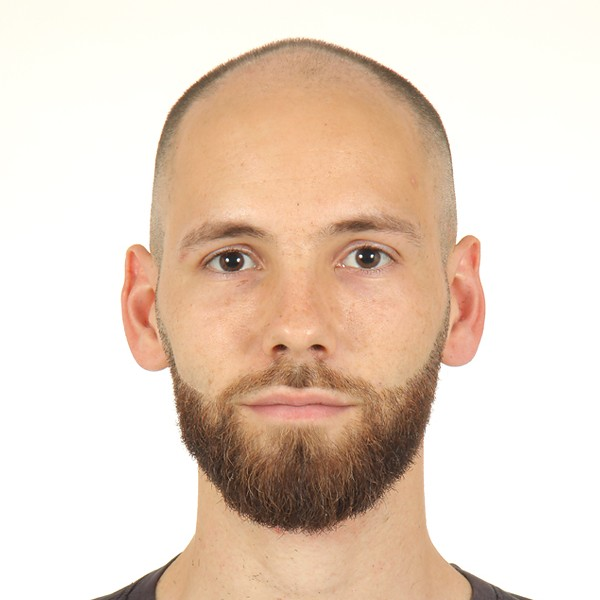
\includegraphics[width=2.8cm, height=2.8cm, keepaspectratio]{foto_carnet2025_cuadrada.jpg}
\end{figure}
\end{minipage} \hfill
\begin{minipage}{0.76\textwidth}
\MyName{Mario Chacón Falcón}
\Websites{\href{https://www.linkedin.com/in/mario-chacon-falcon518831318/}{LinkedIn} $|$ \href{https://github.com/mchacon28}{GitHub} $|$ \href{https://scholar.google.es/citations?user=s39KvDoAAAAJ&hl=es}{Google Scholar} $|$ \href{https://mchacon28.github.io/}{Website}}
\vspace{2mm}
\Websites{Email: \href{mailto:mario.chacon@icmat.es}{mario.chacon@icmat.es} $|$ Affiliation: ICMAT-CSIC / UAM}
\end{minipage}

\vspace{2mm}

%%% 1. Education
\NewPart{Education}

\EducationEntry{Ph.D. Candidate in Mathematics}{2024 - Present}{Instituto de Ciencias Matemáticas (ICMAT) - Universidad Autónoma de Madrid (UAM)}{
Specializing in Bayesian methods, adversarial risk analysis, and multi-agent reinforcement learning. Funded by the European Commission - NextGenerationEU through the Momentum CSIC programme.
}

\EducationEntry{M.S. in Logic, Computation and Artificial Intelligence}{2023 - 2024}{Universidad de Sevilla (Spain)}{
Average grade: \textbf{9.6 / 10}.
}

\EducationEntry{B.S. in Mathematics}{2019 - 2023}{Universidad de Sevilla (Spain)}{
Average grade: \textbf{7.94 / 10}.
}

%%% 2. Academic & Research Appointments
\NewPart{Academic \& Research Appointments}

\WorkEntry{Predoctoral Researcher (Momentum CSIC Programme)}{12/2024 - Present}{Institute of Mathematical Sciences (ICMAT-CSIC)}{
\begin{itemize}
    \setlength\itemsep{0.1em}
    \item Research on Bayesian statistics, adversarial risk analysis, multi-agent reinforcement learning, privacy-preserving federated learning, and decision-theoretic AI security.
    \item Advised by Prof. David Ríos Insua.
\end{itemize}
}

\WorkEntry{Research Fellow (JAE Intro ICU Fellowship)}{01/2024 - 10/2024}{Microelectronics Institute of Seville (IMSE-CNM, CSIC)}{
\begin{itemize}
    \setlength\itemsep{0.1em}
    \item \textbf{Project}: Bio-inspired vision processing systems with deep learning.
    \item Developed and evaluated spiking neural network (SNN) architectures with learnable synaptic delays for neuromorphic spatio-temporal data classification using PyTorch.
\end{itemize}
}

%%% 3. Publications & Preprints
\NewPart{Publications \& Preprints}

\noindent \textbf{Journal articles}
\begin{itemize}
    \setlength\itemsep{0.2em}
    \item \textbf{Privacy-preserving federated learning AdaBoost via knowledge distillation}: \textbf{M. Chacón-Falcón}, J. M. Moyano. \textit{Knowledge-Based Systems}, Vol. 339, Article 116962, 2026. DOI: \href{https://doi.org/10.1016/j.knosys.2026.116962}{10.1016/j.knosys}.
    
    \item \textbf{BAM-SLDK: Biologically inspired attention mechanism with spiking learnable delayed kernel synapses}: \textbf{M. Chacón-Falcón}, A. Patiño-Saucedo, L. Camuñas-Mesa, T. Serrano-Gotarredona, B. Linares-Barranco. \textit{IOP Neuromorphic Computing and Engineering}, Vol. 5, No. 1, 2025. DOI: \href{https://doi.org/10.1088/2634-4386/addb6c}{10.1088/2634-4386/addb6c}.
\end{itemize}

\vspace{0.3em}
\noindent \textbf{Under review and in preparation}
\begin{itemize}
    \setlength\itemsep{0.2em}
    \item \textbf{Adversarial risk analysis with fully probabilistic design}: \textit{Under review at Reliability Engineering \& System Safety (RESS)}.
    
    \item \textbf{Bayesian opponent-aware soft Q-learning}: \textit{In preparation / ongoing research}.
\end{itemize}

%%% 4. Teaching Experience & Training
\NewPart{Teaching Experience \& Training}

\WorkEntry{Instructor / Lecturer}{04/2026}{Escuela de Estadística de las Administraciones Públicas, INE (Madrid, Spain)}{
\begin{itemize}
    \setlength\itemsep{0.1em}
    \item \textbf{Course}: \textit{Introducción a la Estadística Bayesiana} (Introduction to Bayesian statistics).
    \item Taught a 4-hour specialized module on Bayesian foundations, probabilistic modeling, and inference for official statisticians of the Spanish public administrations (course total: 15 teaching hours).
\end{itemize}
}

%%% 5. R&D and Technology Transfer Projects
\NewPart{R\&D and Technology Transfer Projects}

\WorkEntry{Intelligent combat pilot training agent via reinforcement learning}{2024 - 2026}{Airbus Defence and Space SAU \& ICMAT-CSIC}{
\begin{itemize}
    \setlength\itemsep{0.1em}
    \item \textbf{Project}: Development of a training environment based on reinforcement learning models to produce intelligent training agents for combat aircraft pilots.
    \item Research on multi-agent decision-making, simulation dynamics, and robust policy learning in high-stakes adversarial settings.
\end{itemize}
}

\WorkEntry{Intelligence profiling with advanced predictive analytics}{2024 - 2025}{Xeerpa Marketing Solutions, S.L. \& ICMAT-CSIC}{
\begin{itemize}
    \setlength\itemsep{0.1em}
    \item \textbf{Project}: Development of intelligence profiling functionalities using advanced predictive analytics.
    \item Applied machine learning and statistical modeling to user profiling, digital identity analysis, and customer analytics.
\end{itemize}
}

%%% 6. Talks and Conference Presentations
\NewPart{Talks and Conference Presentations}
\begin{itemize}
    \setlength\itemsep{0.2em}
    \item \textbf{Tracking latent goals for robust reinforcement learning}: Contributed talk, II International Workshop on Bayesian Statistics (SEIO Bayesian working group), CUNEF Universidad, Madrid, Spain, June 2026.
    
    \item \textbf{Opponent-aware soft Q-learning}: Oral presentation and discussant in roundtable on adversarial decision making, NextGen Synergy: Control Theory \& Machine Learning (COML 2026 / InterCoML, COST Action CA24136), Prague, Czech Republic, April 2026.
    
    \item \textbf{Towards secure artificial intelligence: Private distributed learning and strategic decision making}: Invited seminar, Institute of Information Theory and Automation (UTIA), Czech Academy of Sciences, Prague, Czech Republic, November 2025.
    
    \item \textbf{Adversarial risk analysis with fully probabilistic designs to handle sequential games}: Oral presentation, EURO 2025 Congress, Leeds, United Kingdom, June 2025. 
    
    \item \textbf{Adversarial risk analysis with fully probabilistic designs}: Oral presentation, XLI SEIO Congress, Lleida, Spain, June 2025.

    \item \textbf{A new federated learning adaptation of AdaBoost}: Conference talk, AEMCO Congress, Sevilla, Spain, September 2024.

    \item \textbf{Delayed SNNs on spatio-temporal neuromorphic datasets}: Poster presentation, AIHUB's Connexion Summer School, Valencia, Spain, July 2024.
\end{itemize}

%%% 7. Academic Service & Leadership
\NewPart{Academic Service \& Leadership}
\begin{itemize}
    \setlength\itemsep{0.2em}
    \item \textbf{Co-organizer}, Reinforcement Learning \& MARL reading group (2026 - Ongoing): Community reading group on mathematical foundations and frontiers of sequential decision-making (\url{https://rl-readinggroup.github.io/}).
    \item \textbf{Co-organizer}, Probabilistic Machine Learning reading group (2025 - 2026): Bi-weekly reading club on advanced Bayesian modeling and inference based on Kevin P. Murphy's textbook (\url{https://pml-reading-club.github.io/}).
\end{itemize}

%%% 8. Languages
\NewPart{Languages}
\begin{itemize}
    \setlength\itemsep{0.2em}
    \item \textbf{Spanish:} Native.
    \item \textbf{English:} Full professional proficiency (C1 / Certificate in Advanced English, Cambridge, Grade B).
\end{itemize}

\end{document}